\documentclass[a4paper,10pt]{article}
\usepackage{fullpage}
\usepackage{float}
\usepackage[english]{babel}
\usepackage{graphicx,subfig,wrapfig}
\usepackage{amsmath,amsfonts,amsthm,amssymb} 
\usepackage{fancyhdr,fancybox,color}
\usepackage{epstopdf}
\usepackage{enumerate}
\usepackage{multirow}
\usepackage[amssymb]{SIunits}             	% SI units package
\definecolor{MyBlue}{rgb}{0,0.3,0.6}      	
\usepackage[colorlinks=true,linkcolor=MyBlue,plainpages=false,citecolor=MyBlue,urlcolor=MyBlue]{hyperref}
\usepackage[all]{hypcap}   					%fixes the hyperref, such that links are anchored at the bottom of the images, not the top
\usepackage[url=false,
backend=bibtex,
style=authoryear-comp,
doi=true,
isbn=true,
backref=false,
dashed=false,
maxcitenames=2,
maxbibnames=99,
natbib=true]{biblatex}
\DeclareNameAlias{author}{last-first}
\renewbibmacro{in:}{}
\addbibresource{../_logosAndRef/references.bib}

\nonfrenchspacing

\begin{document} 
\thispagestyle{empty} % remove the page number on this page

\noindent Chair: Physics of Fluids Department
\begin{center}
 \begin{LARGE}
 Holey sheets: Bursting of liquid films
 \end{LARGE}
\end{center}

\section*{Description}

Droplets in uniform air flow frequently form bag-like structures that ultimately fragment. This fragmentation is critical for understanding several natural and industrial processes, like airborne disease transmission and agricultural pesticide application. 
Although several previous studies have attributed hole formation and subsequent breakup to Van der Waals forces--relevant at molecular scales, many experiments show nucleation in thicker sheets, including those at the micron scale. How can that be? We hypothesize that impurities within liquid sheets, such as bubbles or oil droplets, can trigger hole nucleation at thicknesses much greater than molecular scales. 
Using Basilisk C for direct numerical simulations and employing the Coupled-Level-Set-Volume-of-Fluid and Level-Set methods to resolve interfaces, we elucidate the mechanisms by which these impurities prompt hole formation during sheet drainage. 
We use a simplified axially symmetric radial drainage model, imposing an outward velocity $u = \omega r$, where $\omega$ is the drainage rate, and $r$ is the radial distance (see figure \ref{fig:droplets2021}). This approach captures the essence of bag-like expansion that follows a free-fall like drainage while isolating the hole formation mechanism.
We found that, even when impurities initiate hole formation, the film can heal if the radial driving is weak. Conversely, holes grow and lead to sheet breakup if the imposed flow rate and initial shape distortion are large.
Moreover, smaller cavities consistently heal, whereas larger perturbations always open. Potential chemical or thermal inhomogeneities may further influence these dynamics, delaying hole nucleation. These findings reveal a double threshold for hole formation underlying the role of submicron impurities in droplet fragmentation -- the driving should be strong enough, and the initial shape distortions should be large enough -- refining existing models of droplet breakup and can guide design strategies in aerosol and spray processes.
Several open questions emerge: How do specific impurities or surface agents affect hole formation thresholds? Does local heating or cooling shift the balance between healing and opening? Could non-Newtonian effects or external forcing alter these conclusions? Addressing these questions could refine droplet breakup models and guide future designs in aerosol and spray technologies—offering a rich avenue of study for a bachelor's or master's research project.

\begin{figure}[h]
\centering
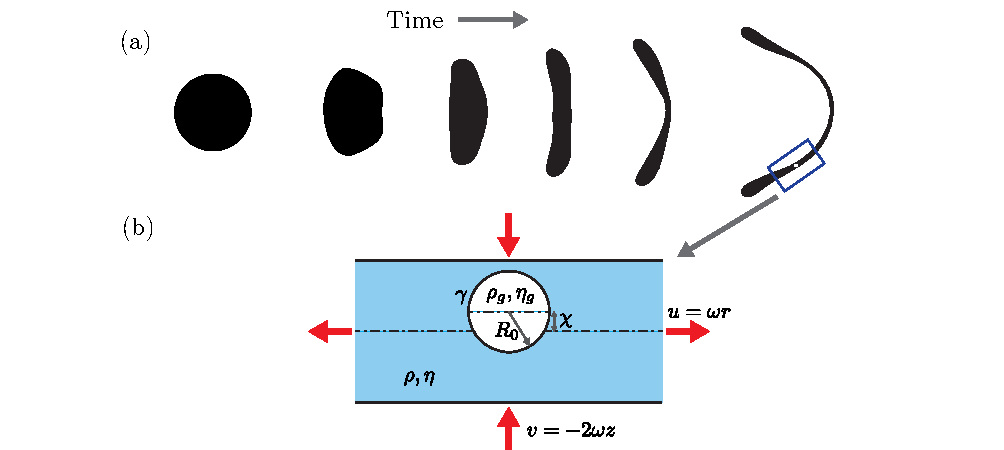
\includegraphics[width=\textwidth]{schematic_02.pdf}
\caption{(a) Droplet in uniform airflow deforms and expands into a bag-like structure. The impurities inside the sheets can prompt breakup when the thickness is of micron order. (b) To model that, bubbles as a defect are simulated inside a simplified two-dimensional liquid draining sheet.}
\label{fig:droplets2021}
\end{figure}

\section*{What you will do and what you will learn?}
In the Physics of Fluids group, we are looking for enthusiastic students to join our newly established project on bursting of sandwiched liquid films.

\begin{enumerate}
\item You will learn about film bursting, Taylor-Culick retractions, and viscous dissipation. 
\item You will work closely with experimentalists. 
\item You will learn about the Computational Fluid Dynamics (CFD) fundamentals, and use the free software program Basilisk C \href{http://basilisk.dalembert.upmc.fr}{(http://basilisk.dalembert.upmc.fr)}.
\item You will have access to a read-to-use codebase (available on \href{https://github.com/comphy-lab/bubbleinSheet}{GitHub}).
\item You will learn how to do basic and advanced scientific data analysis.
\item As a part of the \href{https://comphy-lab.org}{CoMPhy lab}, you will learn and adapt open-source coding principles. 
\end{enumerate}

If you have any questions, feel free to contact \href{mailto:a.k.dixit@utwente.nl}{Ayush} (details below).
\begin{center}
\begin{tabular}{|l|l|l|}
\hline \textbf{Supervision} & \textbf{E-mail} & \textbf{Office} \\
\hline Ayush Dixit M.Sc. & \href{mailto:a.k.dixit@utwente.nl}{a.k.dixit@utwente.nl} & Meander 250 \\
\hline \multirow{2}{*}{Dr. Vatsal Sanjay} & \href{mailto:vatsal.sanjay@comphy-lab.org}{vatsal.sanjay@comphy-lab.org} & \multirow{2}{*}{Durham University} \\
& \href{mailto:vatsal.sanjay@durham.ac.uk}{vatsal.sanjay@durham.ac.uk} & \\
\hline Prof. Dr. Detlef Lohse F.R.S. & \href{mailto:d.lohse@utwente.nl}{d.lohse@utwente.nl} & Meander 261  \\
\hline
\end{tabular}
\end{center}

\printbibliography
\end{document}



